

\documentclass[12pt]{article}
\usepackage{graphicx}
\usepackage{amsmath}
\usepackage{listings}
\usepackage{color}
\usepackage[section]{placeins} %this stops the figures from showing up in wrong section

\definecolor{dkgreen}{rgb}{0,0.6,0}
\definecolor{dkblue}{rgb}{0,0.0,0.6}
\definecolor{dkred}{rgb}{0.9,0.0,0.1}


\begin{document}

\lstset{language=Fortran,tabsize=4,numbers=left,numberstyle=\tiny,basicstyle=\ttfamily\small\color{dkblue},stringstyle=\ttfamily\color{blue},keywordstyle=\rmfamily\color{dkred}\bfseries\emph,backgroundcolor=\color{white},commentstyle=\color{dkgreen}}




\title{Physics 562 - Computational Physics\\[.5cm]
Midterm 4}
\author{Josh Fernandes\\
Department of Physics \& Astronomy\\
California State University Long Beach}
\date{\today}

  
\maketitle



\begin{abstract}
This paper examines two different questions. 
\end{abstract}


\section{Problem 1}

\section{The Fortran95 code}

Numtype is the same for problems 1 and 2. 
\begin{lstlisting}[frame=single,caption={program {\tt gamma.f95}},label=module]

module setup

	use numtype
	implicit none
	integer, parameter :: nsp = 146, npar = 8
	integer :: yy(nsp), minsp, maxsp, iprint, ifcal
	
		
end module setup



program gamma_spectrum

	use setup
	implicit none
	real(dp) :: ii, stuff
	integer :: i, itmin, itmax
	real(dp) :: fstart, xstart(npar), stepi, epsf
	real(dp), external :: least2
	

	open(unit=2, file='Sigma_pion_nucleus.dat')
	open(unit=3, file='Sigma_pion_nucleus.d')
	do i = 1, nsp
		read(3,*) stuff,ii
		write(2,*) ii
		yy(i) = ii
	end do
	close(2)
	close(3)




	minsp = 5
	maxsp = 140
	xstart(1:npar) = (/ -5.01, 0.002, 300000.0, 23.0, 2.0, 150000.0, 60.0,30.0  /)
	
	ifcal = 0
	iprint = 1
	fstart = least2(xstart(1:npar))
	
	itmin = 100
	itmax = 1000
	epsf = 0.001_dp
	stepi = 0.1_dp
	iprint = 0
	
	call downhill(npar, least2, xstart, fstart, stepi, epsf, itmin, itmax)

	iprint = 2
	fstart = least2(xstart(1:npar))


end program gamma_spectrum


function least2(par) result(ss)


	use setup
	implicit none
	real(dp) :: par(npar), a, b, y1, x1, sig1, y2, x2, sig2, ss, fi
	integer :: i


	ifcal = ifcal +1
	a = par(1); b = par(2);
	y1 = par(3);	x1 = par(4);	sig1 = par(5)
	y2 = par(6);	x2 = par(7);	sig2 = par(8)

	ss = 0._dp
	
	do i = minsp, maxsp
		fi = a*i + b + y1*exp(-((i-x1)/sig1)**2) + y2*exp(-((i-x2)/sig2)**2)
		ss = ss + (fi-yy(i))**2/sqrt(yy(i)+1.0)
	end do
	ss = ss/(maxsp-minsp)
	print '(i5,8f12.4, f20.5)', ifcal, par(1:npar), ss
	write(8,*) ifcal, ss
	
	if ( iprint /= 0 ) then
		do i = minsp, maxsp
			fi = a*i + b + y1*exp(-((i-x1)/sig1)**2) + y2*exp(-((i-x2)/sig2)**2)
			write(unit=iprint,fmt='(i4,i10,f15.2)') i,yy(i),fi
		end do

	end if



end function least2



\end{lstlisting}



\section{Problem 2}



\section{The Fortran95 code}

\begin{lstlisting}[frame=single,caption={ {\tt int.f95}},label=module]

program integral

	use numtype
	use integr
	implicit none

	real(dp) :: a,b,c,d,res,eps,ifail,scale
	real(dp), dimension(maxint) :: w_legendre,x_legendre, w_cc, x_cc, &
								   w_lag, x_lag, w_new, x_new
	integer :: nint, itype, i,n_legendre, n_cc, n_lag, n_new
	print *, '================================================================'
	print *, 'Midterm4'

	print *, 'first integration'

	itype = 1
	a = 0._dp
	b = 1._dp
	c = 3/2._dp
	d = 1/2._dp 
	ifail = 0._dp
	n_new = 50._dp

	call d01bcf(itype,a,b,c,d,n_new,w_new,x_new,ifail)

	res = 0._dp
	do i = 1,n_new
		res = res + mid1(x_new(i))*w_new(i)
! 		write(44,*) x_new(i),sqa3(x_new(i))*w_new(i)
	end do
	print *, 'gauss my  value =', res
	print *, 'true value=pi/16=', pi/16
	print *, 'accurate to 15 digits!!!!'

	print *, '================================================================'
	print *, 'Midterm4'

	print *, 'second integration'

	itype = 3
	a = 0._dp
	b = 1._dp
	c = -1/2._dp
	d = 0._dp 
	ifail = 0._dp
	n_new = 50._dp

	call d01bcf(itype,a,b,c,d,n_new,w_new,x_new,ifail)

	res = 0._dp
	do i = 1,n_new
		res = res + mid1(x_new(i))*w_new(i)
! 		write(44,*) x_new(i),sqa3(x_new(i))*w_new(i)
	end do

	print *, '  gauss  my  value =', res
	print *, 'true value=sqrt(pi)=', sqrt(pi)
	print *, 'accurate to 14 digits!!!!'
	


	contains
	
	
			function mid1(x) result(fx)

			real(dp) :: x,fx


			fx = 1

		end function mid1
	

end program integral
	
	
\end{lstlisting}



\section{Results}

\begin {figure}[!htb]
	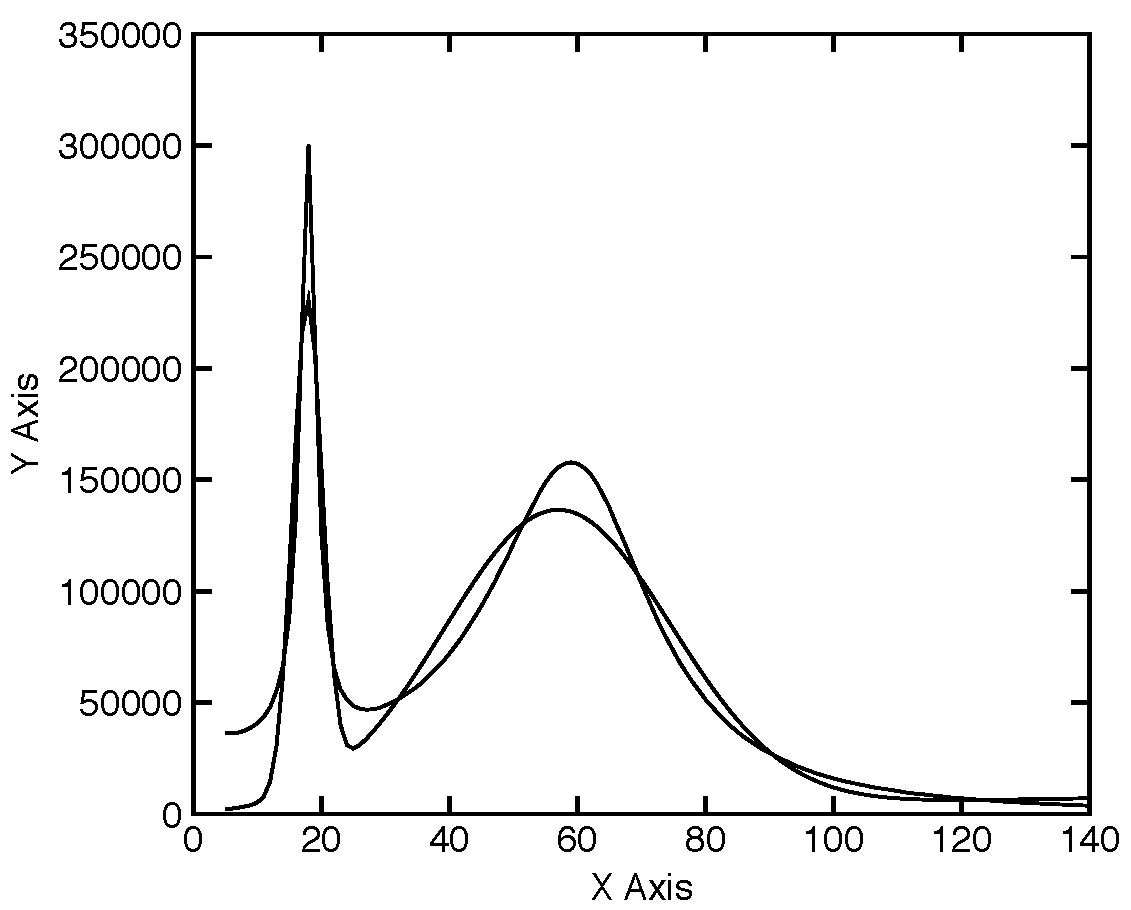
\includegraphics[width=1.\textwidth]{question_1/plot1.pdf}
	%\resizebox{\columnwidth}{!}{\input{question_1/one.png}}
	\caption{first image }
	\label{imageone}
\end {figure}

You can see from Figure 1 that I came up with a fit of the data. E0 should be the energy where the peaks are, which are around 23 and 60. Look at fort.2 in the files to get this graph. The half life should be how fast it decays away, which should be 56.8739 if I am reading terminal correctly.

For question two, the result of the first integral should be $\frac{\pi}{16}$. My value using d01b was $0.19634954084936221$.  For the second integral, the value should be $\sqrt{\pi}$. My value using d01b was $1.7724538509055101$.





\begin{thebibliography}{}


\bibitem{metcalf} M.\ Metcalf, J.\ Reid and M.\ Cohen, {\it Fortran 95/2003 explained}. Oxford University Press, 2004.
 

\end{thebibliography}




\end{document}
